% Начало оглавления. Оно хитро заполняется само, глядя на заголовки
% которые добавляются с помощью \section и \subsection
\renewcommand\contentsname{Оглавление} %%% renaming the Table of Contents
\tableofcontents
\setcounter{page}{2}

\pagebreak
\section*{Введение}
% Такой заголовок пойдет в оглавление, только без нумерации
\addcontentsline{toc}{section}{Введение}


\clearpage
\section{Постановка задачи}

Принцип действия вибрационного погружателя (рис. \ref{fig:scheme_porg}) основан на эффекте резкого снижения сопротивлению погружения свайного элемента при сообщении последнему вибрации. При вращении дисбалансов на их ось крепления действует центробежная сила и вибрационный погружатель получает вибрирующее движение, которое сообщается свайному элементу через наголовник.

\begin{definition}
    Сила, препятствующая материальной точке, движущейся по окружности, удалиться от центра этой окружности, называется центростремительной силой. Она направлена по радиусу от окружности к центру. По третьему закону Ньютона имеется равная ей и противоположно направленная сила противодействия (сила, с которой движущаяся точна стремится удалиться от центра). Эта сила называется центробежной.
\end{definition}

\begin{definition}
    Вибрационным погружением называют внедрение твёрдого тела в сопротивляющуюся среду под действием постоянной и знакопеременной сил.
\end{definition}

% \begin{definition}
%     Под вибрационным внедрением будем понимать внедрение твёрдого тела в сопротивляющуюся среду с заданной средней скоростью.
% \end{definition}

\begin{definition}
    Дебалансом называют неуравновешенность вращающихся частей машин (роторов, коленчатых валов, шкивов и т. п.).
\end{definition}

\begin{figure}[h]
    \centering
    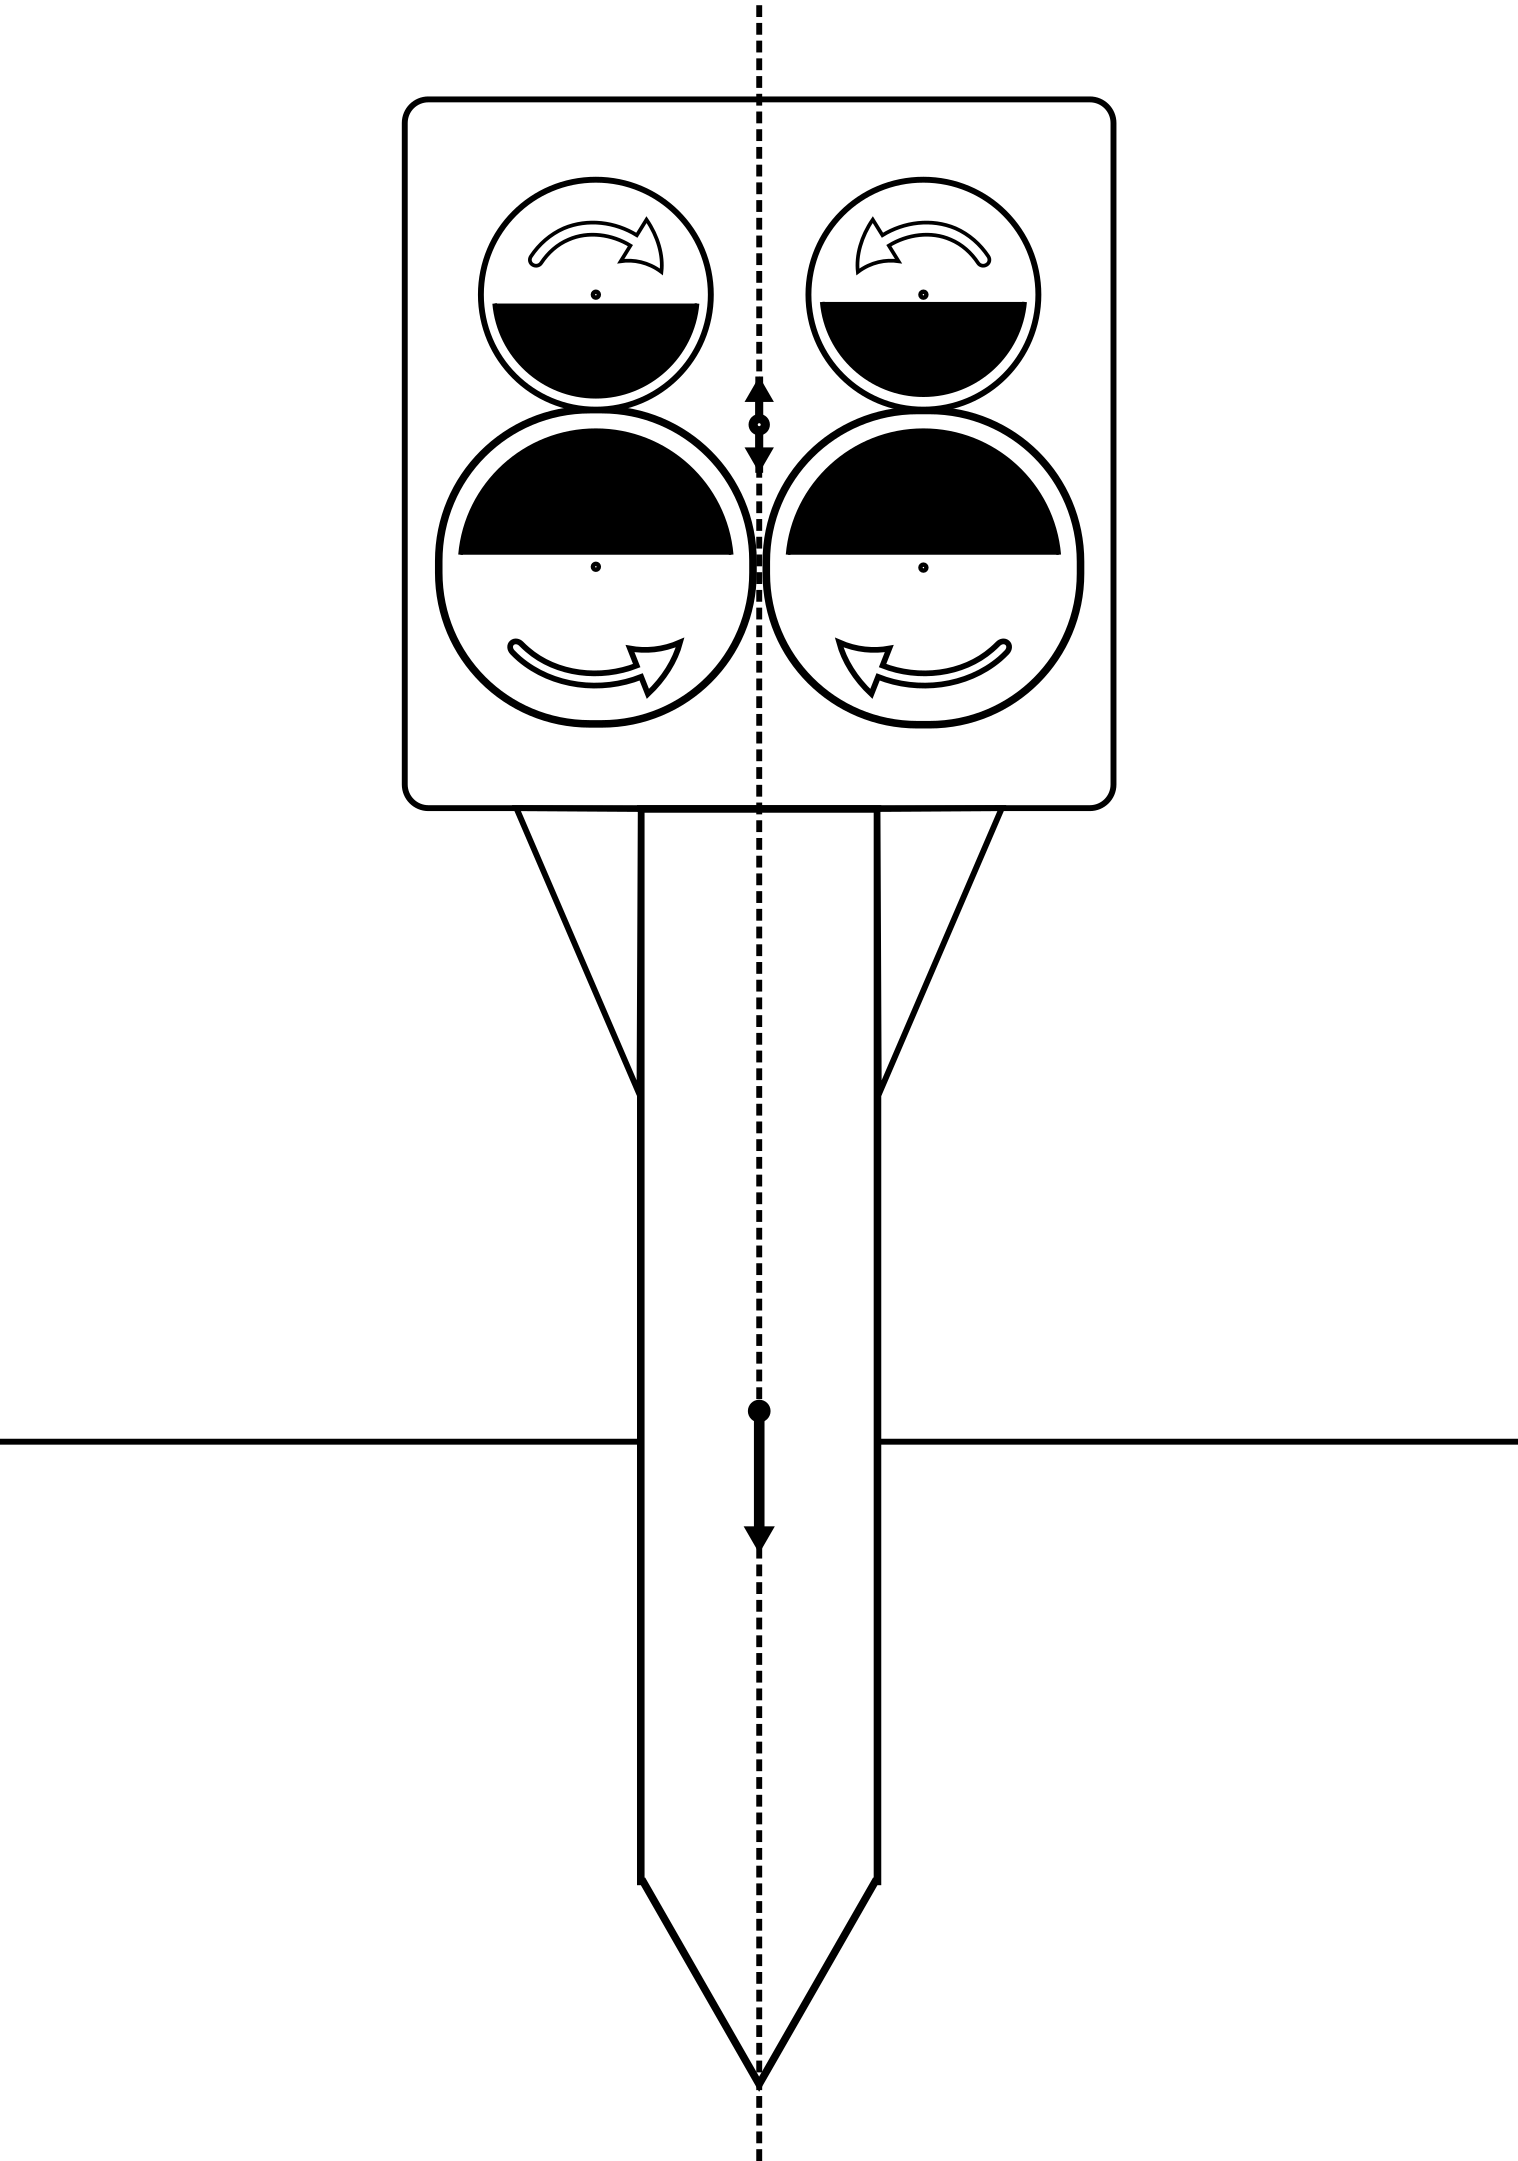
\includegraphics[width=0.5\linewidth]{img/scheme_porg.png}
    \caption{Схема вибрационного погружателя.}
    \label{fig:scheme_porg}
\end{figure}

\begin{definition}
    Сила, препятствующая материальной точке, движущейся по окружности, удалиться от центра этой окружности, называется центростремительной силой. Она направлена по радиусу от окружности к центру. По третьему закону Ньютона имеется равная ей и противоположно направленная сила противодействия (сила, с которой движущаяся точна стремится удалиться от центра). Эта сила называется центробежной.
\end{definition}

\clearpage
\section{Заключение}


\clearpage
\section{Приложение}
\subsection{Исходный код main.py}
% \lstinputlisting[language=Python, breaklines]{code/app.py}


\clearpage
\addcontentsline{toc}{section}{Список литературы}
\begin{thebibliography}{}
    \bibitem{}
\end{thebibliography}

